\section{Space-Time Spectral Analysis}
\label{ch:spectra}

Open from `3.\ Analysis $\to$ Space-Time Spectra`.

The spectral window has four tabs. \textbf{Spatial (Welch)} is always available. \textbf{Temporal} and \textbf{Spatiotemporal} require time-resolved data. \textbf{Spatial (FFT)} is always available and provides a complementary 2D ROI-based spatial spectrum.

\subsection{Spatial Spectra -- Welch (Tab 1)}

The one-dimensional spatial energy spectrum $E(k)$ characterizes the distribution of turbulent kinetic energy across spatial scales. For homogeneous isotropic turbulence, Kolmogorov's similarity theory predicts an inertial subrange where $E(k) \propto k^{-5/3}$ (Kolmogorov, 1941). The spatial spectrum is computed along a user-defined line using Welch's method: the line is divided into overlapping segments, each Hann-windowed and Fourier-transformed, and the periodograms are averaged to reduce variance. The wavenumber $k$ is in rad/m.

```{note}
\begin{enumerate}[leftmargin=1.5em, topsep=2pt]
  \item Choose `Horizontal ($k_x$)` or `Vertical ($k_y$)` mode.
  \item Left-click and drag on the field to draw the line.
  \item Select which velocity components to include (U, V, W).
  \item Set the number of Welch segments and overlap.
  \item Click `Compute`.
\end{enumerate}
```

Results are plotted on a log-log scale. The Kolmogorov $-5/3$ reference slope can be toggled on/off. You can also compensate the spectrum by multiplying by $k^{5/3}$ to flatten the inertial range.

\begin{figure}[htbp]
  \centering
  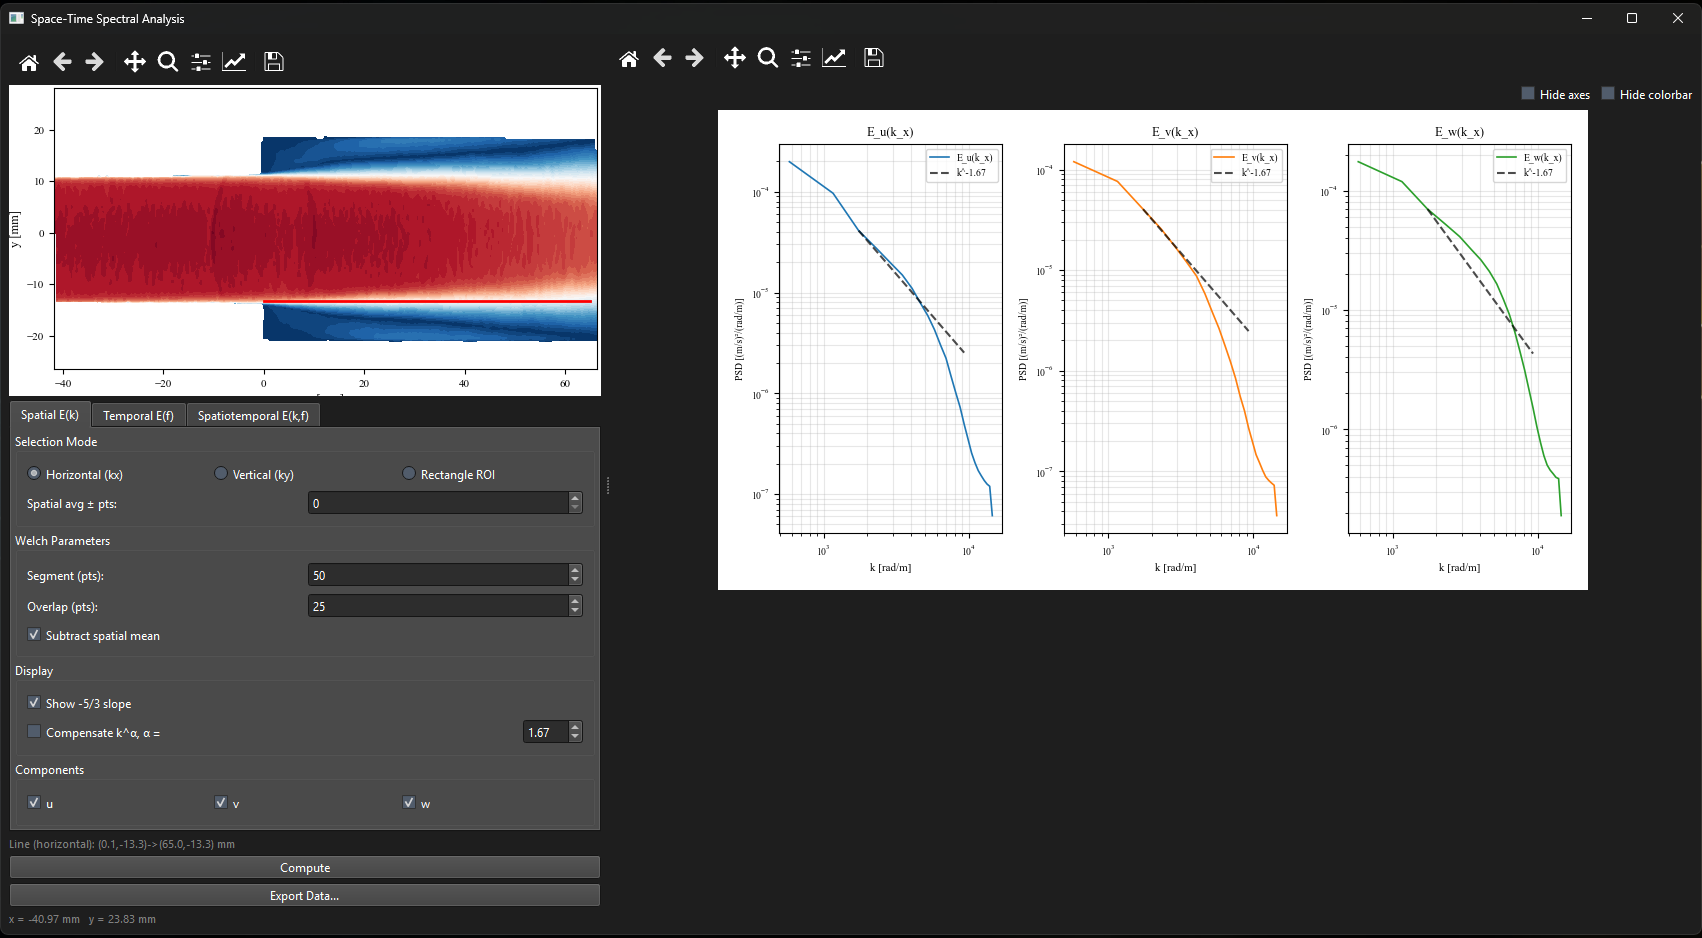
\includegraphics[width=0.92\linewidth]{fig5}
  \caption{Spatial spectra (Welch tab) showing $E(k_x)$ for the U and V components along a horizontal line through the shear layer. The dashed line shows the Kolmogorov $-5/3$ reference slope. The inertial subrange is visible between approximately $k = 100$ and $k = 1000$\,rad/m.}
  \label{fig:spectra}
\end{figure}

\noindent\textbf{Reference:} Kolmogorov, A.N. (1941). The local structure of turbulence in incompressible viscous fluid for very large Reynolds numbers. \textit{Proceedings of the USSR Academy of Sciences}, 30, 301--305.

\subsection{Temporal Spectra (Tab 2, TR Only)}

The power spectral density $E(f)$ of the velocity fluctuations at a fixed point reveals the temporal frequency content of the turbulence. Dominant peaks correspond to periodic or quasi-periodic phenomena such as vortex shedding, shear layer flapping, or acoustic resonances. The temporal spectrum is computed using Welch's method with a Hann window.

```{note}
\begin{enumerate}[leftmargin=1.5em, topsep=2pt]
  \item Left-click on the field to pick a reference point, or right-click drag to draw an ROI.
  \item Set the number of Welch segments. More segments give a smoother spectrum at the cost of frequency resolution.
  \item Click `Compute`.
\end{enumerate}
```

```{tip}
Looking for a shedding frequency or flapping mode? Use fewer segments (higher frequency resolution). Just want the spectral shape? Use more segments for a smoother curve.
```

\subsection{Space-Time Spectra (Tab 3, TR Only)}

The two-dimensional space-time spectrum $E(k, f)$ jointly characterizes the spatial and temporal structure of convecting turbulent structures. It is computed by applying a 2D Fourier transform in both space (along a streamwise line) and time. Diagonal ridges in the resulting map correspond to spatially coherent structures convecting at a fixed speed. The slope of a ridge gives the convection velocity $U_c = 2\pi f / k$, providing a direct test of Taylor's frozen turbulence hypothesis (del Álamo \& Jiménez, 2009).

\noindent\textbf{Reference:} del Álamo, J.C. \& Jiménez, J. (2009). Estimation of turbulent convection velocities and corrections to Taylor's approximation. \textit{Journal of Fluid Mechanics}, 640, 5--26.

\subsection{Spatial Spectra -- FFT (Tab 4)}

Computes the 2D spatial energy spectrum over a rectangular ROI using a direct FFT (via pyFFTW), averaged over all snapshots. The result is shown as 1D marginal spectra $E(k_x)$ and $E(k_y)$ alongside the 2D spectral map.

\subsection{Multi-case comparison}

Spatial Welch and Temporal spectra support CSV import and overlay (Chapter~\ref{ch:multicase}).

% ============================= CHAPTER 8 ==============================
